%%%%%%%%%%%%%%%%%%%%%%%%%%%%%%%%%%%%%%%%%
% Short Sectioned Assignment
% LaTeX Template
% Version 1.0 (5/5/12)
%
% This template has been downloaded from:
% http://www.LaTeXTemplates.com
%
% Original author:
% Frits Wenneker (http://www.howtotex.com)
%
% License:
% CC BY-NC-SA 3.0 (http://creativecommons.org/licenses/by-nc-sa/3.0/)
%
%%%%%%%%%%%%%%%%%%%%%%%%%%%%%%%%%%%%%%%%%

%----------------------------------------------------------------------------------------
%	PACKAGES AND OTHER DOCUMENT CONFIGURATIONS
%----------------------------------------------------------------------------------------

\documentclass[paper=a4, fontsize=11pt]{scrartcl} % A4 paper and 11pt font size

\usepackage[T1]{fontenc} % Use 8-bit encoding that has 256 glyphs
\usepackage{fourier} % Use the Adobe Utopia font for the document - comment this line to return to the LaTeX default
\usepackage[english]{babel} % English language/hyphenation
\usepackage{amsmath,amsfonts,amsthm, amssymb} % Math packages
\usepackage{slashed}

\usepackage{graphicx}
\usepackage{multicol}
\usepackage{enumitem}
\usepackage{caption}
\usepackage{esint}

\usepackage{listings}
\usepackage{color}

\definecolor{dkgreen}{rgb}{0,0.6,0}
\definecolor{gray}{rgb}{0.5,0.5,0.5}
\definecolor{mauve}{rgb}{0.58,0,0.82}

\lstset{frame=tb,
  language=C,
  aboveskip=3mm,
  belowskip=3mm,
  showstringspaces=false,
  columns=flexible,
  basicstyle={\small\ttfamily},
  numbers=none,
  numberstyle=\tiny\color{gray},
  keywordstyle=\color{blue},
  commentstyle=\color{dkgreen},
  stringstyle=\color{mauve},
  breaklines=true,
  breakatwhitespace=true
  tabsize=3
}

\usepackage{lipsum} % Used for inserting dummy 'Lorem ipsum' text into the template

\usepackage{sectsty} % Allows customizing section commands
\allsectionsfont{\centering \normalfont\scshape} % Make all sections centered, the default font and small caps

\usepackage{abstract}
\renewcommand{\abstractnamefont}{\normalfont\Large}
\renewcommand{\abstracttextfont}{\normalfont}

\usepackage{fancyhdr} % Custom headers and footers
\pagestyle{fancyplain} % Makes all pages in the document conform to the custom headers and footers
\fancyhead{} % No page header - if you want one, create it in the same way as the footers below
\fancyfoot[L]{} % Empty left footer
\fancyfoot[C]{} % Empty center footer
\fancyfoot[R]{\thepage} % Page numbering for right footer
\renewcommand{\headrulewidth}{0pt} % Remove header underlines
\renewcommand{\footrulewidth}{0pt} % Remove footer underlines
\setlength{\headheight}{13.6pt} % Customize the height of the header

\numberwithin{equation}{section} % Number equations within sections (i.e. 1.1, 1.2, 2.1, 2.2 instead of 1, 2, 3, 4)
\numberwithin{figure}{section} % Number figures within sections (i.e. 1.1, 1.2, 2.1, 2.2 instead of 1, 2, 3, 4)
\numberwithin{table}{section} % Number tables within sections (i.e. 1.1, 1.2, 2.1, 2.2 instead of 1, 2, 3, 4)

%\setlength\parindent{0pt}  Removes all indentation from paragraphs - comment this line for an assignment with lots of text

%Average
\newcommand{\average}[1]{\ensuremath{\left\langle #1 \right\rangle}}
%Parenthesis 
\newcommand{\parentheses}[1]{\ensuremath{\left( #1 \right)}}
%Commutator
\newcommand{\commutator}[1]{\ensuremath{\left[ #1 \right]}}
%Anti-commutator
\newcommand{\anticommutator}[1]{\ensuremath{\left\lbrace #1 \right\rbrace}}
%QED
\newcommand{\QED}{\begin{flushright}\textit{Q.E.D.}\end{flushright}}
%Split
\newcommand{\spliteq}[1]{\begin{split} #1 \end{split}}
%----------------------------------------------------------------------------------------
%	TITLE SECTION
%----------------------------------------------------------------------------------------

\newcommand{\horrule}[1]{\rule{\linewidth}{#1}} % Create horizontal rule command with 1 argument of height

\title{
\vspace{-2.5cm}
\begin{center}

\includegraphics[width=2.5cm]{logo-kth.png}\\[-1mm]
\hspace{-3mm}
\end{center}
\normalfont \normalsize
\textsc{Theoretical Physics} \\ [25pt] % Your university, school and/or department name(s)
\horrule{0.5pt} \\[0.4cm] % Thin top horizontal rule
\huge GPU Acceleration of the Ising Spin Glass \\ % The assignment title
\Large Advanced Computational Physics\\ % Course name
\Large SI2531, Fall 2014\\ % Course code and Semester
\Large Supervisor: Prof. Mats Wallin \\ %Supervisor
\horrule{2pt} \\[0.5cm] % Thick bottom horizontal rule
}

\author{Jens Wir\'{e}n \\
Farhad Kimanos \\
Stefan Fleischmann \\
\normalsize jenswir@kth.se \\
\normalsize kimanos@kth.se \\
\normalsize sfle@kth.se} % Your name

\date{\normalsize\today} % Today's date or a custom date

\begin{document}

\maketitle % Print the title

%----------------------------------------------------------------------------------------

\begin{abstract}
A two and three dimensional Ising spin glass model with Gaussian couplings on a square lattice is used to study the disordered ground state and obtain the domain wall energy $\Delta E$, by quenching the system from $T=\infty$ to $T=0 K$ for various system sizes. This is used to calculate the critical stiffness exponent $\theta$ from the scaling relation $\Delta E \thicksim L^\theta$ where $L$ is the system size. The results obtained agree well with the known values, $\theta_{2D}=-0.287$ and $\theta_{3D}=0.23$, for two and three dimensions respectively.

The method used is an optimized GPU-accelerated double checker board algorithm written in the Compute Unified Device Architecture (CUDA) language and run on a Nvidia Tesla C2070. The algorithm is benchmarked and computation times are displayed and commented on.
\end{abstract}

\pagebreak

\section{Introduction}

The goal of this simulation is to examine the two-dimensional Ising model defined on a triangular lattice with zero applied field. The Binder cumulant will be used to determine the critical temperature $T_{c}$ and a finite size scaling analysis will be performed to calculate the critical exponents $\nu$ and $\beta$. This will be done both in the ferromagnetic and antiferromagnet case where frustration enters. The results will be compared with the results on a regular square lattice.


\section{Theory}

\subsection{The Ising Model}

The Ising model is one of physics most studied models concerning spin systems. It's both easy to define yet extremely rich in it's behaviour. With small variations the Ising model can describe many interesting systems from the common ferromagnet to the exotic spin glass systems we will alter examine.

The Ising model is defined by the Hamiltonian

\begin{equation}
H = -J \sum\limits_{\left\langle i,j \right\rangle} S_{i} S_{j} -h \sum\limits_{i} S_{i}
\end{equation}
where $S_{i} = \pm 1$ is a spin degree of freedom on lattice site $i$, $\left< i,j \right> $ means nearest neighbour summation, $h$ is an applied magnetic field and $J$ is a coupling
constant. When $J$ is set to $J=+1$ this represents a ferromagnetic and when $J=-1$ an antiferromagnetic.

\subsection{Frustration}
The 2D Ising model defined on a square lattice is the only one with an analytical solution apart from the 1D Ising chain.  Even thou this set up is the easiest in the two-dimensional case the exact solution is very complicated. 

When using ferromagnetic couplings the ground state of this model is simply all spins oriented in the same direction, either up or down. In the antiferromagnetic case it is a checker board pattern of spin up and down. Obviously in both these cases the ground state is non-degenerate. If we define the 2D Ising model on a triangular lattice with ferromagnetic couplings the ground state is still all spin up or down. The antiferromagnetic case however is quite different.

Consider the triangular unit cell and attempt to minimize the energy. Let the top position of the triangle be the first spin, one can orientate this arbitrarily but lets choose up for now. Let the bottom left of the triangle be the second spin and we will now choose this to be down in order to minimize the energy with respect to the first spin. But how is one suppose to orientate the third and final spin located in the bottom right? 

If one chooses this to be spin up we minimize the energy with respect to the second spin but maximize with respect to the first one. If we instead choose spin down the situation is reversed. We can never satisfy the other two spins simultaneously. This means that the ground state of the system will never be as low as for the square lattice or ferromagnetic case. Furthermore the ground state is highly degenerate since there is no unique way to reach it. This phenomenon is known as frustration and is illustrated in Figure \ref{fig:frustration}.

\begin{figure}[hbtp]
\centering
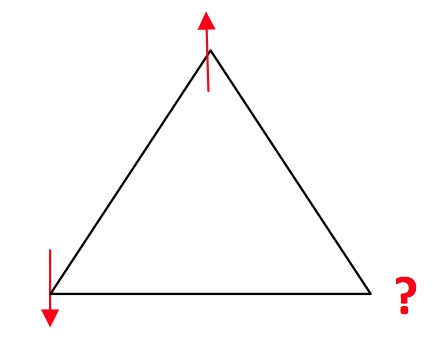
\includegraphics[scale=0.4]{frustration.jpg}
\caption{In the antiferromagnetic 2D Ising model on a triangular lattice there is no way one can orient the spins to minimize all interactions simultaneously.}
\label{fig:frustration}
\end{figure}

\section{Simulation and/or Implementation?}

\section{Results}

\section{Discussion and Conclusions}

\begin{thebibliography}{100}

\bibitem{SVM_book}
Nello Cristianini, John Shawe-Taylor
\emph{An Introduction to Support Vector Machines}.
Cambridge University Press,
1nd Edition,
2000.

\end{thebibliography}
\end{document}

\end{document}